% ============================================================
\section{Actividad 3: Estimación de $H$ en la \textit{European ST-T Database}}
% ============================================================

Se estimó el parámetro de Hurst de la frecuencia cardíaca instantánea
(convertida a BPM desde los intervalos RR) de los $90$ registros de la
\textit{European ST-T Database}, aplicando los estimadores VT y LD.

% ------------------------------------------------------------
\subsection{Resultados por registro}
% ------------------------------------------------------------

\begin{figure}[H]
    \centering
    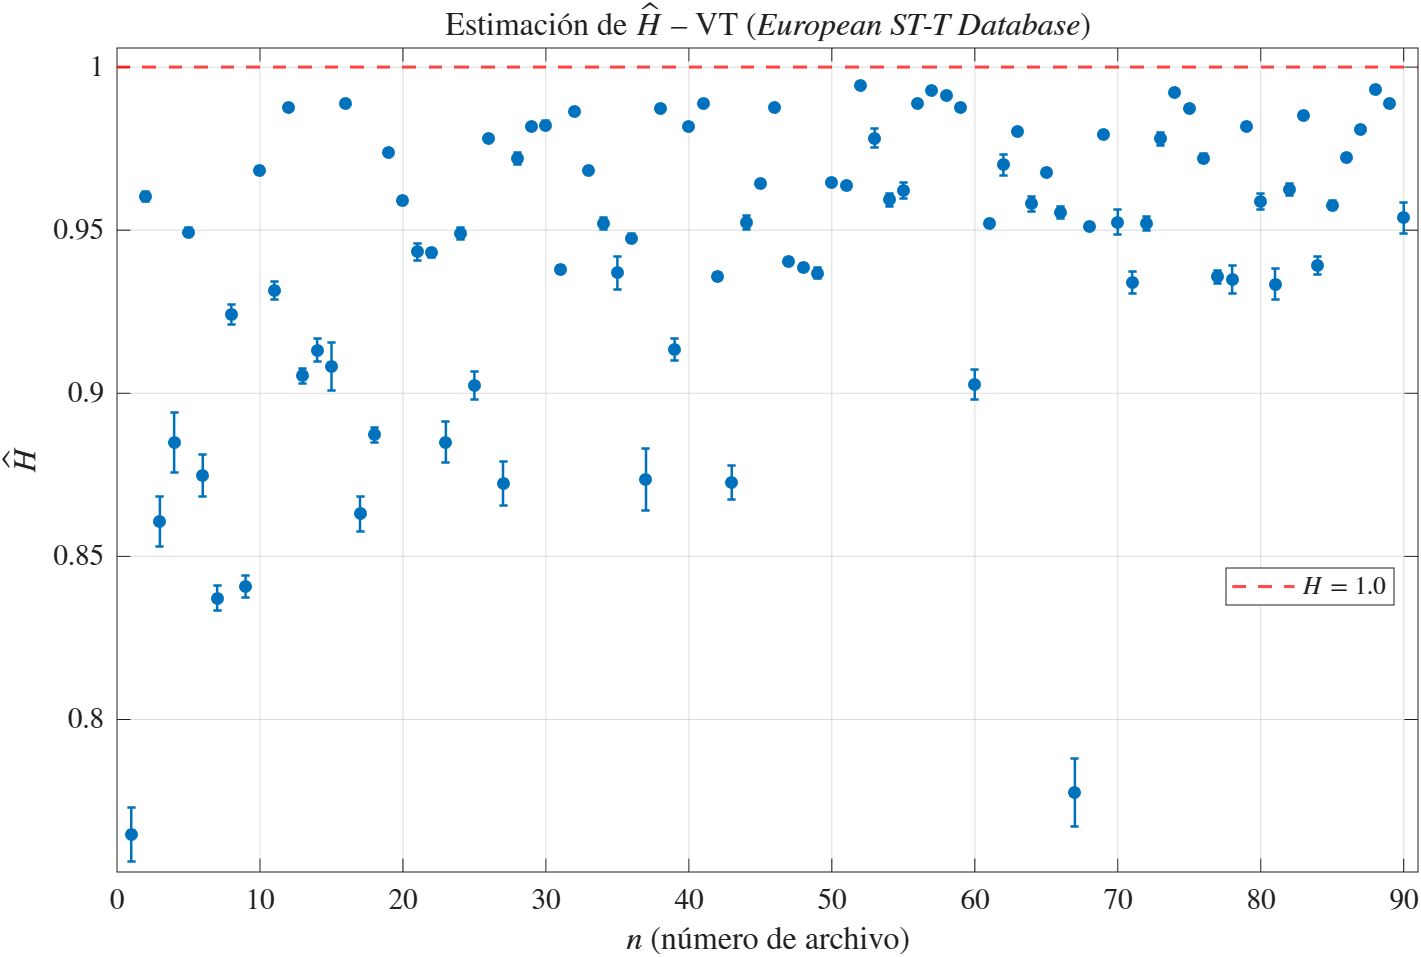
\includegraphics[width=0.95\textwidth]{actividades/actividad3/imgs/errbar_vt.png}
    \caption{Estimación de $\hat{H}$ con VT para los 90 registros,
             con intervalos de confianza $[H_{\min},\, H_{\max}]$.}
    \label{fig:errbar_vt}
\end{figure}

\begin{figure}[H]
    \centering
    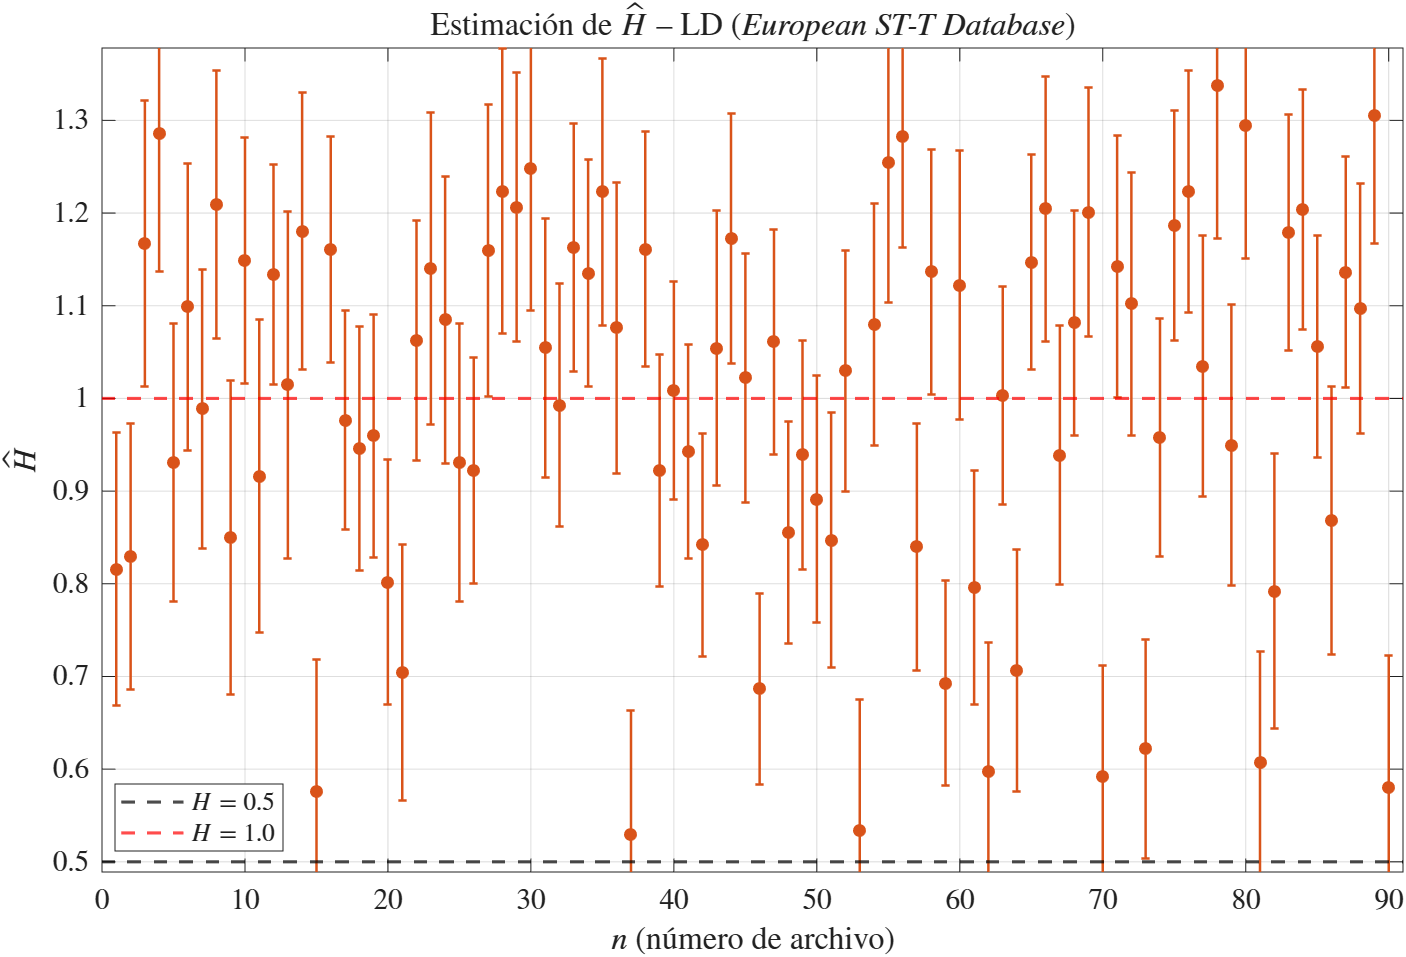
\includegraphics[width=0.95\textwidth]{actividades/actividad3/imgs/errbar_LD.png}
    \caption{Estimación de $\hat{H}$ con LD para los 90 registros,
             con intervalos de confianza $[H_{\min},\, H_{\max}]$.}
    \label{fig:errbar_ld}
\end{figure}

\textbf{Estimador VT (Figura~\ref{fig:errbar_vt}).} Las estimaciones se
concentran en el rango $[0.77,\, 0.99]$, con la mayoría de los registros
entre $0.93$ y $0.98$. Los intervalos de confianza son estrechos y
homogéneos entre registros, lo que se traduce en estimaciones estables y
reproducibles. Dos registros ($n = 1$ y $n = 68$) presentan
$\hat{H} \approx 0.77$, alejándose del comportamiento general. Ninguna
estimación supera $H = 1.0$.

\textbf{Estimador LD (Figura~\ref{fig:errbar_ld}).} Las estimaciones son
notablemente más dispersas: el rango cubre desde $\approx 0.53$ hasta
$\approx 1.29$. Una fracción considerable de registros presenta $\hat{H} > 1.0$,
valor que no tiene interpretación física válida para un proceso estacionario.
Los intervalos de confianza son amplios e inconsistentes entre registros,
con algunos casos cubriendo casi $0.7$ unidades de $H$.

% ------------------------------------------------------------
\subsection{Distribución global}
% ------------------------------------------------------------

\begin{figure}[H]
    \centering
    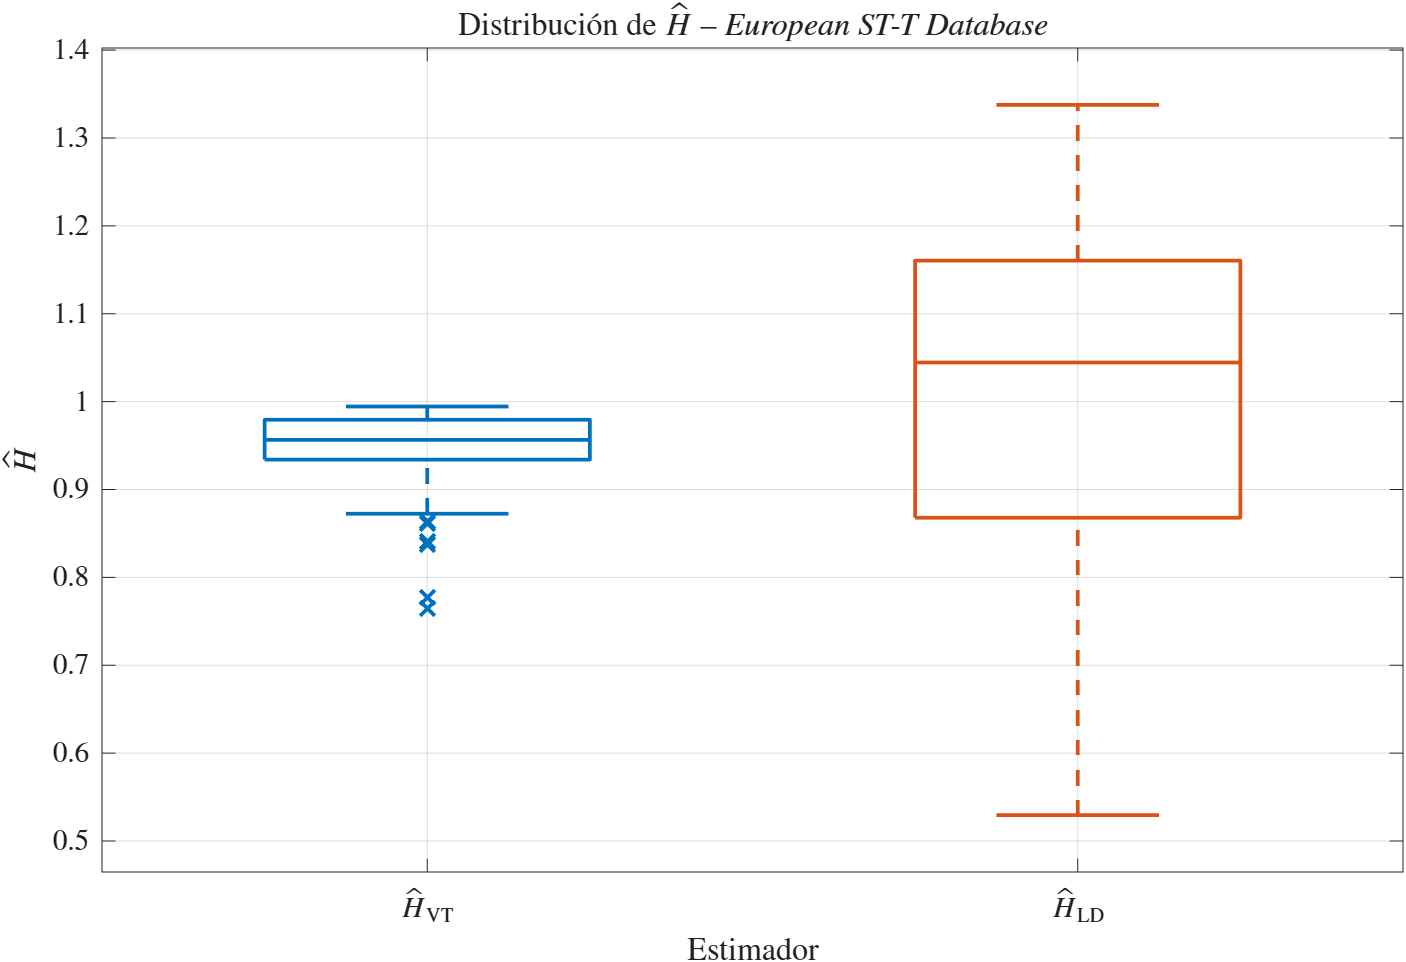
\includegraphics[width=0.80\textwidth]{actividades/actividad3/imgs/qqplot.png}
    \caption{Distribución de $\hat{H}$ para los 90 registros,
             VT (azul) y LD (naranja).}
    \label{fig:boxplot_a3}
\end{figure}

La Figura~\ref{fig:boxplot_a3} resume las diferencias entre estimadores.
En el diagrama de caja y bigotes, el bigote superior representa el valor
máximo no atípico, es decir, el dato más alto que no supera
$Q_3 + 1.5 \cdot \text{IQR}$; el bigote inferior representa el valor mínimo
no atípico, definido como el dato más bajo que no cae por debajo de
$Q_1 - 1.5 \cdot \text{IQR}$. Los puntos fuera de estos límites se
clasifican como valores atípicos y se marcan individualmente.

VT produce una distribución compacta: mediana $\approx 0.96$,
$Q_1 \approx 0.95$, $Q_3 \approx 0.97$, con un rango intercuartílico de
apenas $0.02$. El bigote superior llega a $\approx 1.00$ y el inferior a
$\approx 0.87$, con tres valores atípicos por debajo ($\approx 0.86$,
$0.84$ y $0.77$), que corresponden a registros con dinámica cardíaca
particularmente distinta al resto de la base de datos.

LD presenta mediana $\approx 1.05$, $Q_1 \approx 0.88$, $Q_3 \approx 1.16$,
con un rango intercuartílico casi quince veces mayor que el de VT. El bigote
superior alcanza $\approx 1.34$ y el inferior $\approx 0.53$, sin valores
atípicos detectados. Esto no es una señal favorable: significa que la
dispersión es tan elevada que incluso los valores extremos quedan absorbidos
dentro de los límites estadísticos del diagrama. En VT, los atípicos son
registros genuinamente distintos al resto; en LD, la ausencia de atípicos
refleja que la varianza intrínseca del estimador es tan alta que no permite
distinguir comportamientos excepcionales.

\subsection{Interpretación}

Ambos estimadores coinciden en señalar LRD fuerte en todos los registros
($\hat{H} > 0.5$ en la totalidad de los casos). Sin embargo, sus resultados
difieren sustancialmente en precisión, y la elección del estimador más
adecuado depende de factores que se analizan a continuación.

Los registros de la base de datos contienen del orden de $1\,000$ a $5\,000$
intervalos RR por archivo. En ese régimen de tamaño muestral, la evaluación
sobre secuencias i.i.d.\ demostró que VT presenta menor varianza que LD:
la ventaja de LD en eficiencia solo se materializa para $n \geq 5\,000$.
Este es el argumento más directo para preferir VT en esta base de datos,
independientemente de la naturaleza del proceso.

VT presenta sesgo negativo creciente con $H$: para valores reales cercanos
a $0.9$--$0.95$, subestima el verdadero exponente. Esto sugiere que el valor
real de $H$ podría ser aún más próximo a $1.0$ de lo que reporta. A pesar
de ello, produce estimaciones estrechas y físicamente interpretables
($\hat{H} < 1.0$) en la totalidad de los registros.

LD genera en varios registros $\hat{H} > 1.0$, valor sin interpretación
física válida para un proceso estacionario. Esto no refleja una propiedad
real de la señal, sino la alta varianza de LD cuando opera en el régimen
de alta LRD con muestras de tamaño moderado. La ausencia de valores atípicos
en su boxplot no es favorable: evidencia que su dispersión intrínseca es tan
elevada que incluso los valores extremos resultan estadísticamente normales
dentro de su distribución.

Cabe señalar que la adecuación definitiva de cada estimador a esta señal
depende también de su naturaleza mono o multifractal, cuestión que se aborda
en la Actividad 4. Si la señal resultara monofractal y de tamaño muestral
suficiente, LD podría ofrecer ventajas adicionales en eficiencia.

En conclusión, para esta base de datos y en las condiciones actuales de
tamaño muestral, VT produce estimaciones más confiables: $\hat{H}_{\text{VT}}
\approx 0.96$ como valor central, con baja dispersión entre registros y
coherencia física garantizada. Los resultados de LD deben interpretarse con
cautela.